\documentclass[runningheads,a4paper]{llncs}

\usepackage{amssymb}
\setcounter{tocdepth}{3}
\usepackage{graphicx}
\usepackage{tikz}
\usepackage[T1]{fontenc}
\usepackage[scaled]{beramono}
\usepackage{listings}
\usepackage{color}
\usetikzlibrary{arrows,chains,positioning,scopes,quotes,calc}
\usepackage{float}

\newcommand{\keywords}[1]{\par\addvspace\baselineskip
\noindent\keywordname\endspace\ignorespaces#1}
\pagestyle{plain}
\setlength\parindent{0pt}

\definecolor{mygreen}{RGB}{28,172,0} % color values Red, Green, Blue
\definecolor{mylilas}{RGB}{170,55,241}

\newcommand*{\StrikeThruDistance}{0.15cm}%
\newcommand*{\StrikeThru}{\StrikeThruDistance,\StrikeThruDistance}%

\tikzset{strike thru arrow/.style={
    decoration={markings, mark=at position 0.5 with {
        \draw [blue, thick,-] 
            ++ (-\StrikeThruDistance,-\StrikeThruDistance) 
            -- ( \StrikeThruDistance, \StrikeThruDistance);}
    },
    postaction={decorate},
}}

\lstset{
  language=Python,
  showstringspaces=false,
  formfeed=\newpage,
  tabsize=4,
  commentstyle=\itshape,
  basicstyle=\ttfamily,
  morekeywords={models, lambda, forms}
}

\begin{document}

\mainmatter  % start of an individual contribution

% This needs some work, big time.
\title{Worlds.db: a Proveably Fair Database}

\author{Ryan Walker\\
				ryan.cjw@gmail.com}

\institute{} %Merp

\maketitle

\begin{abstract}
This paper outlines how to move a traditional trusted database into the
decentralized world. This yealds the advantege of using existing database
structure, ie: SLQ and Mongo - without having to reinvent the world.
\end{abstract}

\section{Worlds}
\subsection{Introduction}
Before I start, I should say there are several centralised components of this
y architecture. However I chosen to build it's implementation as a ``phase zero''
of Worlds. 
\\


Blockchain infrastructure is being used to build decentralised games. However
most games are build using traditional database infrasture. Building technology
has always been about getting to market fast, building your MVP first and the
focusing on the core tech once the world realised it's capabilities. Most gaming
projects in the space have moved straight to the ideal without answering the core
question of: How will you get gamers?
\\


The anwer to the questions is simple, you need to build incrediable games. Execution
on the answer is not simple, the gaming market is dominated by huge companies. Unless
you have a silver bullet of a game, you're going to be hard pressed to drive adoption.
\\

The quickest way to drive adoption is to take existing MMO infrastrucutre and build
around it. This is why I chose to write the document. I will outlinine how to
port traditional databases to reach a near trustless entity,

\subsection{Overview}
Nearly all MMO games are using a traditional databsese. This is SQL, Mongo or otherwise.
These databases rely on a trusted design, meaning whoever hosts the database will not 
commit to malicious activity. However there is a way to build a ecosystem that relies
on a central database without having to trust the contents.
\\

This is called distributed verification, the contents on the datbase are verified on
a blockchain, with the heavy lifting done by the database. This also has the added 
feature of not having to port existing games to having blockchain interaction.

\subsection{Archatecture}

\subsubsection{Existing Design}
The existing deign shown in figure whatever is the obvious solutions to a MMO game.
The data is kept in a normal trusted database.

\begin{figure}[H]
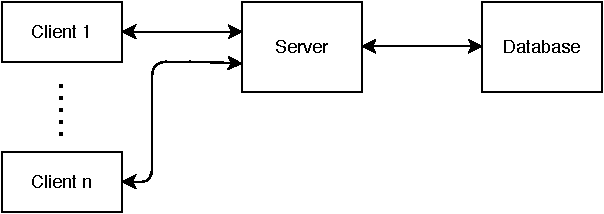
\includegraphics[scale=1]{img/traditional.pdf}
\end{figure}

\subsubsection{Existing Design}
The existing deign shown in figure whatever is the obvious solutions to a MMO game.
The data is kept in a normal trusted database.

\begin{figure}[H]
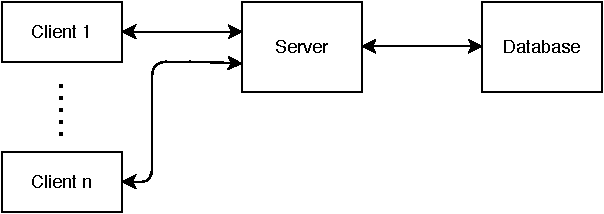
\includegraphics[scale=1]{img/traditional.pdf}
\end{figure}




The archatecutre is laid out in figure 1. The clients connect to the


\end{document}

